\documentclass[tikz,border=6pt]{standalone}
\usepackage[T1]{fontenc}
\usepackage{textcomp}
\usepackage{lmodern}
\usepackage{amssymb}
\newcommand{\q}{\textquotesingle}
\usetikzlibrary{positioning,arrows.meta,calc,fit}

\newcommand{\Nat}{$\mathbb{N}$}

\begin{document}
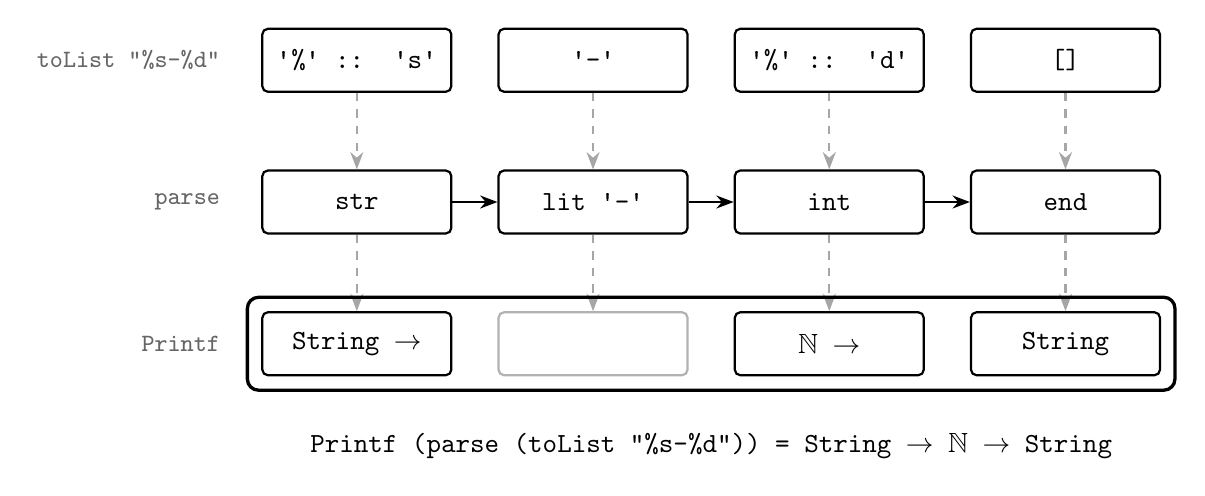
\begin{tikzpicture}[
    >={Stealth[length=2.2mm]},
    box/.style={draw, thick, rounded corners=2pt, minimum width=24mm,
                minimum height=8mm, font=\ttfamily},
    ghost/.style={box, draw=gray!60, text=gray!70},
    row/.style={font=\ttfamily\small, anchor=east, text=gray!80!black},
    map/.style={->, thick, gray!70, dashed},
  ]
  \def\dx{3.0}

  % row 1: characters of the format string
  \node[box] (c1) at (0*\dx,  0) {\q\%\q{} :: \q{}s\q};
  \node[box] (c2) at (1*\dx,  0) {\q-\q};
  \node[box] (c3) at (2*\dx,  0) {\q\%\q{} :: \q{}d\q};
  \node[box] (c4) at (3*\dx,  0) {[]};

  % row 2: parsed Format
  \node[box] (f1) at (0*\dx, -1.8) {str};
  \node[box] (f2) at (1*\dx, -1.8) {lit \q-\q};
  \node[box] (f3) at (2*\dx, -1.8) {int};
  \node[box] (f4) at (3*\dx, -1.8) {end};

  % row 3: Printf contribution
  \node[box]   (t1) at (0*\dx, -3.6) {String $\to$};
  \node[ghost] (t2) at (1*\dx, -3.6) {};
  \node[box]   (t3) at (2*\dx, -3.6) {\Nat{} $\to$};
  \node[box]   (t4) at (3*\dx, -3.6) {String};

  % row labels
  \node[row] at ($(c1.west)+(-0.4,0)$) {toList "\%s-\%d"};
  \node[row] at ($(f1.west)+(-0.4,0)$) {parse};
  \node[row] at ($(t1.west)+(-0.4,0)$) {Printf};

  % vertical mapping
  \foreach \i in {1,...,4} {
    \draw[map] (c\i) -- (f\i);
    \draw[map] (f\i) -- (t\i);
  }

  % Format nesting: each constructor holds the rest
  \foreach \i/\j in {1/2, 2/3, 3/4}
    \draw[->, thick] (f\i) -- (f\j);

  % result
  \node[box, fit=(t1)(t4), inner sep=5pt, draw, very thick, rounded corners=4pt,
        minimum height=0pt] (all) {};
  \node[font=\ttfamily, below=4mm of all]
    {Printf (parse (toList "\%s-\%d")) = String $\to$ \Nat{} $\to$ String};
\end{tikzpicture}
\end{document}
